\documentclass[tikz,border=2pt]{standalone}
% Preámbulo común de los diagramas TikZ (misma paleta y letra que las notas)
\usepackage[T1]{fontenc}\usepackage[utf8]{inputenc}
\usepackage{libertinus}\usepackage{libertinust1math}
\usepackage[defaultsans,scale=0.92]{lato}
\usepackage{amsmath,amssymb,bm}
\usepackage{tikz}\usetikzlibrary{calc,positioning,arrows.meta,shapes.geometric,decorations.pathreplacing,decorations.pathmorphing,fit,backgrounds}
\definecolor{snlazul}{HTML}{1E5AA8}\definecolor{snlnoche}{HTML}{14213D}\definecolor{snlvioleta}{HTML}{6C4AB6}
\definecolor{snlcoral}{HTML}{D1495B}\definecolor{snlambar}{HTML}{E09F3E}\definecolor{snlverde}{HTML}{2A9D8F}
\definecolor{snlteal}{HTML}{0F7173}\definecolor{snlgris}{HTML}{5C677D}\definecolor{snlfondo}{HTML}{F4F6FA}
\tikzset{>={Stealth[length=2.2mm]},
  bloque/.style={draw=#1,fill=#1!8,thick,rounded corners=2pt,minimum height=11mm,minimum width=20mm,align=center,font=\small},
  bloque/.default=snlazul,
  suma/.style={draw=snlnoche,thick,circle,inner sep=0pt,minimum size=5mm},
  flecha/.style={->,thick,draw=snlnoche},
  etq/.style={font=\small,text=snlnoche},
  nota/.style={font=\footnotesize\sffamily,text=snlgris,align=center}}

\begin{document}
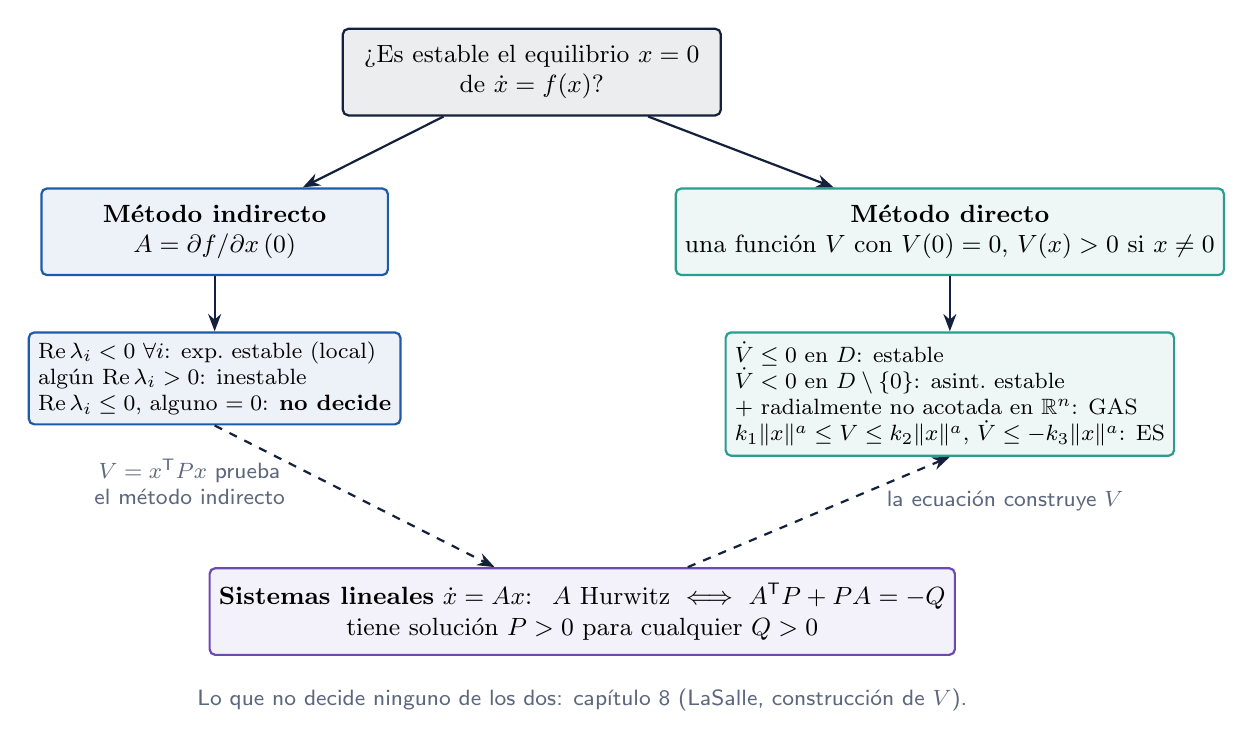
\begin{tikzpicture}[node distance=6mm and 8mm]
 \node[bloque=snlnoche,minimum width=48mm] (q) {¿Es estable el equilibrio $x=0$\\ de $\dot x=f(x)$?};
 \node[bloque=snlazul,below left=9mm and -6mm of q,minimum width=44mm] (ind) {\textbf{Método indirecto}\\ $A=\partial f/\partial x\,(0)$};
 \node[bloque=snlverde,below right=9mm and -6mm of q,minimum width=48mm] (dir) {\textbf{Método directo}\\ una función $V$ con $V(0)=0$, $V(x)>0$ si $x\neq0$};
 \node[bloque=snlazul,below=7mm of ind,minimum width=44mm,align=left,font=\footnotesize] (indr) {$\operatorname{Re}\lambda_i<0$ $\forall i$: exp.\ estable (local)\\ algún $\operatorname{Re}\lambda_i>0$: inestable\\ $\operatorname{Re}\lambda_i\le0$, alguno $=0$: \textbf{no decide}};
 \node[bloque=snlverde,below=7mm of dir,minimum width=48mm,align=left,font=\footnotesize] (dirr) {$\dot V\le0$ en $D$: estable\\ $\dot V<0$ en $D\setminus\{0\}$: asint.\ estable\\ $+$ radialmente no acotada en $\mathbb R^n$: GAS\\ $k_1\|x\|^a\le V\le k_2\|x\|^a$, $\dot V\le-k_3\|x\|^a$: ES};
 \node[bloque=snlvioleta,below=16mm of $(indr.south)!0.5!(dirr.south)$,minimum width=70mm] (lin) {\textbf{Sistemas lineales} $\dot x=Ax$: \ $A$ Hurwitz $\iff$ $A^{\mathsf T}P+PA=-Q$\\ tiene solución $P>0$ para cualquier $Q>0$};
 \draw[flecha] (q) -- (ind); \draw[flecha] (q) -- (dir);
 \draw[flecha] (ind) -- (indr); \draw[flecha] (dir) -- (dirr);
 \draw[flecha,dashed] (indr.south) -- node[pos=0.4,left=4mm,nota]{$V=x^{\mathsf T}Px$ prueba\\ el método indirecto} (lin);
 \draw[flecha,dashed] (lin) -- node[pos=0.6,right=4mm,nota]{la ecuación construye $V$} (dirr.south);
 \node[nota,below=3mm of lin] {Lo que no decide ninguno de los dos: capítulo~8 (LaSalle, construcción de $V$).};
\end{tikzpicture}
\end{document}
